
\documentclass[runningheads]{llncs}
%

%\usepackage{amsmath}
\usepackage{amssymb}
%\usepackage{amsthm}


\usepackage{graphicx}


% Used for displaying a sample figure. If possible, figure files should
% be included in EPS format.
%
% If you use the hyperref package, please uncomment the following line
% to display URLs in blue roman font according to Springer's eBook style:
% \renewcommand\UrlFont{\color{blue}\rmfamily}

\newcommand{\tup}[1]{{\langle #1 \rangle}}
\newcommand{\pre}{\mathsf{pre}}    % precondition
\newcommand{\eff}{\mathsf{eff}}    % effect
\newcommand{\cond}{\mathsf{cond}}  % condition
\newcommand{\dur}{\mathsf{dur}}    % duration
\newcommand{\obs}{\mathsf{obs}}    % observation
\newcommand{\start}{\mathsf{start}}% start
\newcommand{\en}{\mathsf{end}}     % end
\newcommand{\til}{\mathsf{til}}    % TIL
\newcommand{\supp}{\mathsf{sup}}   % sup
\newcommand{\tim}{\mathsf{time}}   % time
\newcommand{\reqs}{\mathsf{req\_{start}}} % req_start
\newcommand{\reqe}{\mathsf{req\_{end}}}   % req_end
\newcommand{\ini}{\mathsf{init}}   % init
\newcommand{\goal}{\mathsf{goal}}  % goal



\begin{document}

\title{One-Shot Learning of Temporal Action Models with Constraint Programming}


\titlerunning{CP to Learn Temporal Planning Models}
% If the paper title is too long for the running head, you can set
% an abbreviated paper title here
%
\author{Antonio Garrido \and Sergio Jim\'enez}

\authorrunning{A. Garrido, S. Jim\'enez}
% First names are abbreviated in the running head.
% If there are more than two authors, 'et al.' is used.
%
\institute{Universitat Polit\`ecnica de Val\`encia \\ Camino de Vera s/n. 46022 Valencia, Spain
\\ \email{\{agarridot,serjice\}@dsic.upv.es}}

\maketitle              % typeset the header of the contribution

\begin{abstract}
Otros titulos:  Learning Temporal Planning Models from Partial Observability by using Constraint Programming; On the Application of Constraint Programming to Learning and Validating;
Learning Temporal Planning Models from Partial Observability of Plan Executions

The paper shows that existing CSP compilations for temporal planning can be adapted to build action models for temporal planning.


150--250 words.

3 Mayo abstract
10 mayo full paper 15 pages (references not included)
Paper: 15 pages

Application track - scheduling, rostering and planning;
Incluso en Testing and Verification como segunda opción

\keywords{Learning action models \and Temporal planning \and Constraint programming.}
\end{abstract}


\section{Introduction}
\label{sec:introduction}

{\em Automated planning} is the model-based approach for the task of selecting actions that achieve a given set of goals starting from a given initial state. {\em Classical planning} is the vanilla model for automated planning and it assumes: fully observable states under a deterministic world, instantaneous actions, and goals that are exclusively referred to the last state reached by a plan~\cite{geffner2013concise,ghallab2004automated}. Beyond classical planning, there is a bunch of more expressive planning models that relax the previous assumptions to compute more detailed solutions than classical plans~\cite{ghallab2004automated}.

{\em Temporal planning} is one of these more expressive planning models, as it relaxes the assumption of {\em instantaneous actions}~\cite{fox2003pddl2}. Temporal actions have durations and their corresponding conditions/effects that must hold/happen at different times, which means that temporal actions can be executed in parallel and overlapping in several ways~\cite{cushing2007temporal}. Consequently, valid solution plans for temporal planning problems indicate the precise time-stamp when an action starts and ends~\cite{howey2004val}.

Despite the performance and potential of state-of-the-art planners, its applicability to real-world tasks is still somewhat limited because of the complexity of specifying correct and complete planning models~\cite{kambhampati2007model}. The more expressive the planning model is, the more evident becomes this knowledge acquisition bottleneck, which jeopardizes the usability of AI planning technology. This has led to a growing interest in the automated planning community for the learning of action models~\cite{jimenez2012review}. The objective of this learning task is to compute action models (i.e. identifying the action's conditions and effects) that are {\em consistent} with a set of observations (defined as some sequence of state changes, world transitions, expert demonstrations or plan traces/logs). Model learning from observation of past behaviour provides indirect, but very valuable information to hypothesize the action models, thus helping future planning decisions and recommendations. This is specially interesting for proactive assistants when recognizing activities of (human or software) agents to assist them in their daily activities and, as the last frontier, to predict and anticipate their needs or actions.

Machine Learning approaches for the learning of planning action models typically follows an inductive learning approach. The main inconvenient of this approach is that usually requires large datasets of observations e.g., thousands of plan observations to compute a statistically significant model by minimizing some error metric over the observations~\cite{yang2007learning,MouraoZPS12,zhuo2013action,kuvcera2018louga}. Defining model learning as an optimization task over a set of observations does not guarantee completeness (the model may not explain all the observations) nor correctness (the states induced by the execution of the plan generated with the model may contain contradictory information). This paper analyses the application of {\em Constraint Programming} for the {\em one-shot learning} of temporal action models that is, the extreme case of learning planning action models from a single observation sample and proposes a simple but effective CSP formulation to learn temporal planning models regarding the partial observations of the execution of an input temporal plan. 

While learning an action model for classical planning means to identify which are the action's conditions and effects that are consistent with a set of partial observations, the learning a temporal action model extends this to (1), identify how these conditions and effects are temporally distributed within the action execution and (2), estimate the actions duration. As a motivating example, let us assume a logistics plan trace. Loosely speaking, learning the temporal planning model will allow us: i) to better understand the insights of the logistics scenario in terms of what is possible (or not) and why, because the model is consistent with the observed data; ii) to suggest changes that can improve the model originally created by a human, e.g. re-distributing the action's conditions, provided they still explain the observations; and iii) to automatically elaborate similar models for similar scenarios, such as public transit for commuters, tourists or people in general in metropolitan areas (\emph{a.k.a.} smart urban mobility). 

Learning the classical action model has been addressed by different approaches~\cite{arora2018review} but, to our knowledge, none learns the temporal features. This means that observations may refer to the executions of concurrent actions which makes our approach suitable for learning in multi-agent environments. Further, the paper evidences that the learning of action models strongly resembles the task of synthesizing and validating a plan that is consistent with the input observations. Our work assumes that input observations are noiseless, meaning that if a value is observed, then the observation is correct. Further, despite the aimed temporal action model is unknown, a set of possible action models (defined as a partially specified action model) is already known and given as input.


%contributions aqui o en conclusiones??
%The paper is organized as follows...


\section{Background}
\label{sec:background}

This section formalizes the {\em classical} and {\em temporal} planning models we use in the paper as well as the {\em Constraint Satisfaction Problem}, the general framework we follow to formulate our learning task.

\subsection{Classical Planning}
\label{sec:classicalplanning}

{\em States} are represented with a set $F$ of propositional variables. A state $s$ is a full assignment of values to fluents, $|s|=|F|$. Without loss of generality, we assume that $F$ does not contain conflicting values $f$ and $\neg f$.

A {\em classical planning problem} is a tuple $\tup{F,I,G,A}$, where $I$ is a total assignment of the state variables representing the initial state, $G \subseteq F$ is a set of goal conditions over the state variables, and $A$ is the set of actions for updating the state variables. We assume that actions are grounded from given action schemas or operators, as in PDDL (Planning Domain Definition Language~\cite{fox2003pddl2}).

Each {\em action} $a \in A$ has a set of preconditions $\pre(a)$ and a set of effects; $\pre(a), \eff(a) \subseteq F$ s.t., $\pre(a)$ must hold before $a$ starts (this is why they are named \emph{pre}conditions), whereas $\eff(a)$ happen when $a$ ends. This way, $a$ is applicable in a state $s$ if $\pre(a) \subseteq s$. When $a$ is executed, a new state, the successor of $s$, is created that results of applying $\eff(a)$ on $s$. Typically, $\eff(a)$ is formed by positive and negative/delete effects. Fig.~\ref{fig:exampleactions}-top shows an example of two classical actions.

A {\em classical plan} is a set of pairs $\tup{(a_1,s_1),(a_2,s_2)\ldots (a_n,s_n)}$. Each $(a_i,s_i)$ pair contains an instantaneous action $a_i$ and the planning step $s_i$ when $a_i$ starts and ends. Classical plans can be sequential plans, where only one action is executed at each planning step, or parallel plans, where several actions can be executed at the same planning step. {\em A solution} to a classical planning problem is a plan such that its execution, starting from the initial state, reaches a final state where goals are satisfied. 

\subsection{Temporal Planning}
\label{sec:temporalplanning}

A {\em temporal planning problem} is a tuple $\tup{F,I,G,A}$ where $F$, $I$ and $G$ are defined like in the classical planning problem, and $A$ represents the set of {\em durative actions}. There are several options that allow for a high expressiveness of durative actions. An action can have a fixed duration, a duration that ranges within an interval or a distribution of durations (time is usually modeled in $\mathbb{R}^+$). Similarly, actions may have conditions/effects at different times, such as conditions that must hold some time before the action starts, effects that happen just when the action starts, in the middle of the action or some time after the action finishes~\cite{garrido2009constraint}.

The planning community uses the slightly restrictive temporal definition of durative actions introduced in PDDL2.1~\cite{fox2003pddl2}, which defines a durative action as follows:
\begin{itemize}
\item $\dur(a)$, a positive value for the action duration.
\item $\cond_s(a), \cond_o(a), \cond_e(a) \subseteq F$. Unlike the \emph{pre}conditions of a classical action, now conditions must hold before $a$ ({\em at start}), during the entire execution of $a$ ({\em over all}) or when $a$ finishes ({\em at end}), respectively.
\item $\eff_s(a)$ and $\eff_e(a)$. Now effects can happen {\em at start} or {\em at end} of $a$, respectively, and can still be positive or negative.
\end{itemize}

Despite durative actions are no longer instantaneous in PDDL2.1, {\em at start} and {\em at end} conditions are checked instantaneously. In the same way, {\em at start} and {\em at end} effects are instantaneously applied ---continuous effects are not considered. With this regard, the semantics of a durative action can be defined in terms of two discrete events, $\start(a)$ and $\en(a)=\start(a)+\dur(a)$.
{\em Over all} conditions must hold at any state between $[\start(a)..\en(a)]$. Fig.~\ref{fig:exampleactions}-bottom shows an example of two durative actions.

PDDL2.2 is an extension of PDDL2.1 that includes the notion of Timed Initial Literal~\cite{hoffmann2005} ($\til(f,t)$), as a way of defining a fact $f$ (literal) that becomes true at a certain time $t$, independently of the actions in the plan. TILs are useful to define exogenous happenings; for instance, a time window when a warehouse is open in a logistics scenario ($\til(open,8)$ and $\til(not-open,20)$).

A temporal plan is a set of pairs $\tup{(a_1,t_1),(a_2,t_2)\ldots (a_n,t_n)}$. Each $(a_i,t_i)$ pair contains a durative action $a_i$ and induces two discrete events, $t_i=\start(a_i)$ and $t_i+\dur(a_i)=\en(a_i)$. Though a sequential temporal plan is syntactically possible, it is semantically useless. Consequently, temporal plans are always given as parallel plans.

\begin{figure}
\caption{Operators that define the schema for two classical and PDDL2.1 durative actions, respectively, for a logistics scenario from the International Planning Competition (IPC, \texttt{http://www.icaps-conference.org/index.php/Main/Competitions}). This is part of the \emph{driverlog} domain, where \texttt{board-truck} boards a driver on an empty truck at a given location, with a fixed duration. In \texttt{drive-truck} a driver drives a truck between two locations, provided there is a link between them (the duration depends on the locations).}

\begin{tabular}{p{\textwidth}}
\begin{verbatim}
(:action board-truck
  :parameters (?d - driver ?t - truck ?l - location)
  :precondition (and (at ?d ?l) (empty ?t) (at ?t ?l) )
  :effect (and (not (at ?d ?l)) (not (empty ?t)) (driving ?d ?t)))
(:action drive-truck
  :parameters (?t - truck ?from - location ?to - location ?d - driver)
  :precondition (and (at ?t ?from) (link ?from ?to) (driving ?d ?t))
  :effect (and (not (at ?t ?from)) (at ?t ?to)))
\end{verbatim}

\begin{verbatim}
(:durative-action board-truck
  :parameters (?d - driver ?t - truck ?l - location)
  :duration (= ?duration 2)
  :condition (and (at start (at ?d ?l)) (at start (empty ?t))
                  (over all (at ?t ?l)))
  :effect (and (at start (not (at ?d ?l))) (at start (not (empty ?t)))
               (at end (driving ?d ?t))))
(:durative-action drive-truck
  :parameters (?t - truck ?from - location ?to - location ?d - driver)
  :duration (= ?duration (driving-time ?from ?to))
  :condition (and (at start (at ?t ?from)) (at start (link ?from ?to))
                  (over all (driving ?d ?t)))
  :effect (and (at start (not (at ?t ?from))) (at end (at ?t ?to))))
\end{verbatim}
\end{tabular}
\label{fig:exampleactions}
\end{figure}


\subsection{The observation model}
\label{sec:omodel}
From the trace of a temporal plan we can optionally extract a set of partial observations $\tup{\obs(f_1,t_1),\obs(f_2,t_2)\ldots \obs(f_n,t_n)}$, where each $\obs(f_i,t_i)$ denotes the value observed for fact $f_i \in F$ at time $t_i$. Note that we work with partial observability of the temporal plan, as we observe only a few facts at certain times. Obviously, the observability of all facts at all actions' starting/ending times would lead to a full observability of the plan state trajectory.

Given a set of propositional variables $F$, a set of {\em durative actions} $A$ and an observation $\mathcal{O}=\tup{s_0^o,s_1^o \ldots , s_m^o}$ of the execution of a temporal plan within these two sets given planning frame, then $P_\mathcal{O}$ is the temporal planning problem that is built as follows $P_\mathcal{O}=\tup{F,A,s_0^o,s_m^o}$. 

\begin{definition}[Explanation]
We say that a plan $\pi$ {\em explains} $\mathcal{O}$ iff $\pi$ is a solution for $P_\mathcal{O}$ that is {\em consistent} with the state trajectory constraints imposed by the sequence of partial states $\mathcal{O}$. 
\end{definition}

The {\em observation} $\mathcal{O}$ is then a sequence of ordered {\em landmarks} for the $P_\mathcal{O}$ classical planning problem~\cite{hoffmann2004ordered}, because all the literals in the observation must be achieved by any plan that solves $P_\mathcal{O}$ and in the same order as are defined in the observation $\mathcal{O}$.


\subsection{Constraint Satisfaction Problem}
\label{sec:csp}

A Constraint Satisfaction Problem is defined as the triple $\tup{V,D,C}$, where:

\begin{itemize}

\item $V=\tup{v_0,v_1 \ldots v_n}$ is a set of $n$ finite domain variables.

\item $D=\tup{D_{v_0},D_{v_1} \ldots D_{v_n}}$ are the respective domains defining the set of possible values for each variable $v \in V$.

\item $C=\tup{c_0,c_1 \ldots c_m}$ is a set of n-ary constraints binding the possible values of the variables in $V$.

\end{itemize}

An evaluation of values to variables is consistent if it does not violate any of the constraints in $C$. Such an evaluation is a solution for a given CSP if it includes values for all the variables while keeping the consistency.


\section{Learning Temporal Models. A Simple Task?}
%\subsection{Preliminary Notes on Learning Temporal Models}
\label{sec:preliminarynotes}

%A priori, learning a temporal action model does not seem to differ a lot from learning a classical action model.

Once we have learned the preconditions+effects of a classical action, learning a temporal action model may seem, a priori, a straightforward task as it \emph{just} implies to distribute the conditions+effects in time and estimate durations. However, this is untrue.

\begin{figure}

%Plan trace: \\
%$\start(a): a; \pre(a); \eff(a)$ \\
%$2: a1; \pre(a1)=\{\}; \eff(a1)=\{p,r\}$ \\
%$4: a2; \pre(a2)=\{\}; \eff(a2)=\{p,q\}$ \\
%$7: a3; \pre(a3)=\{r\}; \eff(a3)=\{not-p\}$ \\
%$10: a4; \pre(a4)=\{p,q,r\}; \eff(a4)=\{not-r\}$ \\

\center 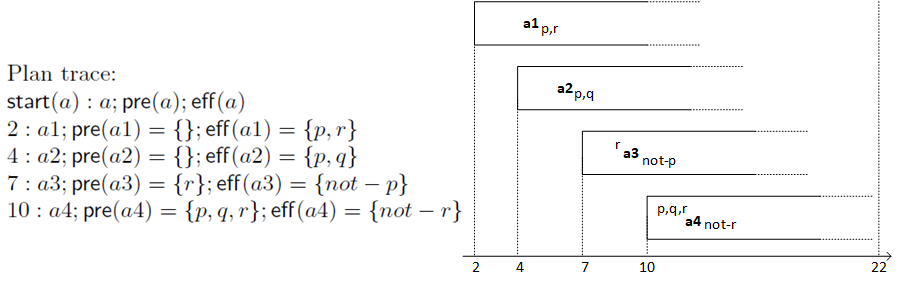
\includegraphics[width=12cm]{ejemploacciones2.png}
\caption{A simple example of how learning a temporal action model is not straightforward. We know the plan makespan is 22, but depending on the distribution of conditions, effects and durations, many situations are possible, though some of them inconsistent.}
\label{fig:exampleplantrace}
\end{figure}


Let us suppose the plan trace of Fig.~\ref{fig:exampleplantrace}, with the preconditions, effects and start times of actions. Clearly, $a3$ needs $a1$ to have $r$ supported, which represents the causal link or dependency $\tup{a1,r,a3}$. Let us imagine that $r$ is in $\cond_s(a3)$. In such a case, if $r$ is in $\eff_s(a1)$, $\dur(a1)$ is irrelevant to $a3$, but if $r$ is in $\eff_e(a1)$, $\dur(a1)$ has to be lower or equal than 5 ($\start(a1)+\dur(a1) \leq \start(a3)$). On the contrary, if $r$ is in $\cond_e(a3)$, $\dur(a1)$ could be much longer. Therefore, the distribution of conditions and effects has a significant impact in the durations, and vice versa.

$a4$ needs $p$, which means two possible causal links ($\tup{a1,p,a4}$ or $\tup{a2,p,a4}$). The real causal link will be the last to happen, and this depends on the effects+durations of $a1$ and $a2$. Therefore, the causal links are unknown, not easy to detect and they affect the structure of the temporal plan. But $a4$ really needs both $a1$ and $a2$ to have $p,q,r$ supported. Let us imagine that $p,q,r$ are in $\cond_s(a4)$ and $p,q$ in $\eff_e(a2)$; then $\dur(a2) \leq 6$. Even if we knew for sure that $\dur(a2)=6$ and $r$ was in $\eff_e(a1)$, we could never estimate the exact value of $\dur(a1)$, as any value in $]0..8]$ would be valid. Intuitively, an action has to wait until the last of its supports, but we cannot grant when the other supports happen; those supporting times and respective durations can never be assured. Therefore, in some situations the precise duration cannot be found and we can only provide values that make the model consistent.

On the other hand, $a3$ deletes $p$, which means that it might \emph{threat} the causal link $\tup{a1,p,a4}$ or $\tup{a2,p,a4}$. But again, this threat depends on the distribution of conditions+effects and the durations. For instance, if $not-p$ is in $\eff_s(a3)$, then $a1$ or $a2$ must support $p$ after time 7 and before $a4$ requires it, which entails many consistent alternatives. On the contrary, if $p$ is in both $\eff_s(a1)$ and $\eff_s(a2)$, this plan trace is inconsistent as $a3$ deletes $p$ and no other action in the plan supports $p$ for $a4$. However, if $not-p$ is in $\eff_e(a3)$, $\dur(a3) > 3$ and $p$ is in $\cond_s(a4)$, then no threat will occur in the plan. Therefore, causal links and threats can easily appear or disappear depending on the selected distributions and durations.

Finally, there are some philosophical questions without a clearly motivated answer. First, why some conditions are modeled as \emph{at start} and others as \emph{over all}? In the temporal version of \texttt{drive-truck} of Fig.~\ref{fig:exampleactions}, why \texttt{(driving ?d ?t)} is required throughout the entire action but \texttt{(link ?from ?to)} only at its beginning? Apparently, the link between the two locations should remain all over the driving; so is this a wrong decision of the human modeler?
Second, why some effects are modeled as \emph{at start} and others as \emph{at end}? In \texttt{board-truck}, why is \texttt{(not (empty ?t))} happening at start and \texttt{(driving ?d ?t)} at end? Could it be in the opposite way?
Third, what happens if one action requires/supports what it deletes (see $a4$ in Fig.~\ref{fig:exampleplantrace}, which might threat itself)? In such a case, the delete effect should happen later than its requirement/supporting.
Four, what happens if all effects are \emph{at start}? This makes little sense, as the duration of the actions would be undetermined and could potentially exceed the known plan horizon or makespan no matter the problem goals. In Fig.~\ref{fig:exampleplantrace}, if the effects of $a1$ and $a2$ are \emph{at start}, is it sensible to allow their durations to pass the limit of 22? In other words, once all plan goals are achieved, can the actions be executed beyond the plan makespan or they need to be cut off to such a value? This decision could potentially lead to an infinite number of models and overlapping situations, so it is not commonly accepted.

As can be noticed from above, learning a temporal action model is not simple. Many possible combinations are feasible provided they fit the constraints the model imposes. Consequently, formulating a CSP from a plan trace and finding a consistent solution that explains that formulation seems an appealing and very promising approach to learn temporal models.



\section{A Constraint Programming Formulation to Learn Temporal Planning Models}
\label{sec:CPformulation}

The underlying idea is to create a single CSP formulation that includes all the constraints a temporal plan trace imposes: i) the actions' conditions, effects, start times and durations; ii) the causal structure of the plan with the supports, to avoid threats and possible contradictory effects; iii) the TILs, if exist; and iv) the optional known observations. Our formulation, inspired in the work by \cite{garrido2009constraint}, is solver-independent. This means that any CSP solver that supports the expressiveness of our formulation, with binary and non-binary constraints, can be used.

\subsection{Variables and domains}

For simplicity, and to deal with integer variables, we model time in $\mathbb{Z}^+$. In order to prevent time from exceeding the plan horizon, we bound all the times to the makespan of the plan\footnote{We use the makespan, which is known from the plan trace, to restrict the duration of the actions. However, this is dispensable if we consider a long enough domain for durations.}.
For each action $a$ in the plan trace, we create the variables represented in Table~\ref{table:variables}. Variables define the time-stamps for actions, the causal links, the interval when conditions must hold and the time when the effects happen.

Our temporal model formulation is more expressive than PDDL2.1 (see more details in section~\ref{sec:PDDL21constraints} below), and allows conditions and effects to be at any time, even outside the execution of the action. For instance, let us imagine a condition $p$ that only needs to be maintained for 5 time units before an action $a$ starts (e.g. warming-up a motor before driving): the expression $\reqe(p,a)=\start(a); \reqe(p,a) = \reqs(p,a)+5$ is possible in our formulation. Additionally, we can represent an effect $p$ that happens in the middle of action $a$: $\tim(p,a) = \start(a)+ (\dur(a) / 2)$ is also possible.



\begin{table}
\begin{center}
\small
\begin{tabular}{p{2cm}p{2.7cm}p{7.4cm}}
\textbf{Variable} & \textbf{Domain} & \textbf{Description} \\

\hline

%\multicolumn{3}{l}{Vars. necessary for action times} \\

$\start(a)$ & \emph{known value} & start time of $a$ given in the plan trace \\
$\dur(a)$ & $[1..makespan]$ & duration of $a$. Optionally, it can be bounded by $makespan-\start(a)$\\
$\en(a)$ & \emph{derived value} & end time of $a$: $\en(a)=\start(a)+\dur(a)$ \\

%\multicolumn{3}{l}{Vars. necessary for action conditions+effects} \\

$\supp(p,a)$ & $\{b_i\}$ that \newline supports $p$ & symbolic variable for the set of potential supporters $b_i$ of condition $p$ of $a$ (causal link $\tup{b_i,p,a}$) \\

$\reqs(p,a)$, \\
$\reqe(p,a)$ & $[0..makespan]$ & interval $[\reqs(p,a)..\reqe(p,a)]$ at which action $a$ requires $p$ \\

$\tim(p,a)$ & $[0..makespan]$ & time when effect $p$ of $a$ happens \\


\hline
\end{tabular}
\normalsize
\end{center}
\caption{Formulation of variables and their domains.}
\label{table:variables}
\end{table}


In addition to actions of the plan trace, we create two dummy actions $\ini$ and $\goal$ for each planning problem $\tup{F,I,G,A}$. First,
$\ini$ represents the initial state $I$ ($\start(\ini)=0$ and $\dur(\ini)=0$). $\ini$ has no variables $\supp, \reqs$ and $\reqe$ because it has no conditions. $\ini$ has as many $\tim(p_i,\ini)=0$ as $p_i$ in $I$.
Second, $\goal$ represents $G$ ($\start(\goal)=makespan$ and $\dur(\goal)=0$). $\goal$ has as many $\supp(p_i,\goal)$ and $\reqs(p_i,\goal)=\reqe(p_i,\goal)=makespan$ as $p_i$ in $G$. $\goal$ has no variables $\tim$ as it has no effects.


One interesting benefit of our formulation is that it allows us to model TILs and observations exactly like other actions. On the one hand, $\til(f,t)$ can be seen as a dummy action ($\start(\til(f,t))=t$ and $\dur(\til(f,t))=0$) with no conditions and only one effect $f$ that happens at time $t$ ($\tim(f,\til(f,t))=t$). A $\til$ is analogous to $\ini$, as they both represent information that is given at a particular time, but externally to the execution of the plan.
On the other hand, $\obs(f,t)$ can be seen as another dummy action ($\start(\obs(f,t))=t$ and $\dur(\obs(f,t))=0$) with only one condition $f$, which is the value observed for fact $f$, and no effects at all. An $\obs$ is analogous to $\goal$, as they both represent conditions that must be satisfied in the execution of the plan at a particular time.



\subsection{Constraints}

Constraints define relationships among the variables of Table~\ref{table:variables}, thus making it possible the learning process from the plan trace.
The three first constraints are intuitive enough. The fourth constraint models the causal links. Note that in a causal link $\tup{b_i,p,a}$, $\tim(p,b_i) < \reqs(p,a)$ and not $\leq$. This is because temporal planning assumes an $\epsilon > 0$ as a small tolerance between the time when an effect $p$ is supported and when it is required~\cite{fox2003pddl2}. Since we model time in $\mathbb{Z}^+$, $\epsilon=1$. This is the reason why $\en(a) < \start(\goal)$ and not $\leq$; two consecutive actions need to be separated by an $\epsilon$.
The fifth constraint avoids any threat via promotion or demotion~\cite{ghallab2004automated}. The sixth constraint models the fact the same action requires and deletes $p$. Note here the $\geq$ inequality; this is possible because if one condition and one effect of $a$ happen at the same time, the underlying semantics considers the condition is always checked before the effect. The seventh constraint solves the fact that two (possible equal) actions have contradictory effects.

It is important to note that constraints involve any type of actions. Consequently, $\ini$, $\goal$, $\til$ and $\obs$ are subsumed in this formulation.


\begin{table}
\begin{center}
\small
\begin{tabular}{p{5cm}p{7.1cm}}
\textbf{Constraint} & \textbf{Description} \\

\hline

$\en(a)=\start(a)+\dur(a)$ & end time of $a$ \\

$\en(a) < \start(\goal)$ & any action must end before $\goal$ \\

$\reqs(p,a) \leq \reqe(p,a)$ & [$\reqs(p,a)..\reqe(p,a)$] must be a valid interval \\

\begin{tabular}{l}
if $\supp(p,a)=b_i$ then \\
\hspace{0.2cm}$\tim(p,b_i) < \reqs(p,a)$
\end{tabular}
& modeling causal link $\tup{b_i,p,a}$: the time when $b_i$ supports $p$ must be before $a$ requires $p$ \\

\begin{tabular}{l}
$\forall b_j \neq a$ that deletes $p$ at time $\tau_j$: \\
\hspace{0.2cm}if $\supp(p,a)=b_i$ then \\
\hspace{0.4cm}$\tau_j < \tim(p,b_i)$ OR \\
\hspace{0.4cm}$\tau_j > \reqe(p,a)$
\end{tabular}
& solving threat of $b_j$ to causal link $\tup{b_i,p,a}$ being $b_j \neq a$\\

\begin{tabular}{l}
if $a$ requires and deletes $p$: \\
\hspace{0.2cm}$\tim(not-p,a) \geq \reqe(p,a)$ \\
\end{tabular}
& when $a$ requires and deletes $p$, the effect happens after the condition \\

\begin{tabular}{l}
$\forall a_i,a_j \mid a_i$ supports $p$ and \\
\hspace{1.2cm}$a_j$ deletes $p$: \\
\hspace{0.2cm}$\tim(p,a_i) \neq \tim(not-p,a_j)$ \\
\end{tabular}
& solving effect interference ($p$ and $not-p$): they cannot happen at the same time \\

\hline
\end{tabular}
\normalsize
\end{center}
\caption{Formulation of constraints.}
\label{table:constraints}
\end{table}



\subsection{Specific Constraints for Durative Actions of PDDL2.1}
\label{sec:PDDL21constraints}


As described in section~\ref{sec:temporalplanning}, PDDL2.1 restricts the expressiveness of temporal planning in terms of conditions, effects, durations and structure of the actions. Our temporal formulation is significantly richer than PDDL2.1, but adding constraints to make it fully PDDL2.1-compliant is straightforward.


First, $((\reqs(p,a) = \start(a))$ OR ($\reqs(p,a) = \en(a)))$ AND $((\reqe(p,a) = \start(a))$ OR ($\reqe(p,a) = \en(a)))$ limits condition $p$ to be \emph{at start}, \emph{over all} or \emph{at end}, i.e. $p$ is in $\cond_s(a)$, $\cond_o(a)$ or $\cond_e(a)$, respectively.
Further, if a condition is never deleted in a plan, it can be considered as an invariant condition for such a plan. In other words, it represents static information. This type of condition is commonly used in planning to ease the grounding process from the operators; e.g. to model that there is a link between two locations and, consequently, a driving is possible, or modeling a petrol station that allows a refuel action in a given location, etc. Therefore, the constraint to be added for an invariant condition $p$ is simply: $((\reqs(p,a) = \start(a))$ AND $(\reqe(p,a) = \en(a)))$, i.e. $p \in \cond_o(a)$.
Surprisingly, invariant conditions are modeled differently depending on the human modeler. See, for instance, \texttt{(link ?from ?to)} of Fig.~\ref{fig:exampleactions}, which is modeled as an \emph{at start} condition despite: i) no action can be planned to delete that link, and ii) the link should be necessary all over the driving.
This also happens in the \emph{transport} domain of the IPC, where a refuel action requires to have a petrol station in a location only \emph{at start}, rather than \emph{over all} which makes more sense. This shows that modeling a planning domain is not easy and it highly depends on human's decision. On the contrary, our formulation checks the invariant conditions and deals with them always in the same coherent way.


Second, $((\tim(p,a) = \start(a))$ OR $(\tim(p,a) = \en(a)))$ makes an effect $p$ happen only \emph{at start} or \emph{at end} of action $a$, i.e. $p$ is in $\eff_s(a)$ or $\eff_e(a)$.
Also, if all effects happen \emph{at start} the duration of the action would be irrelevant and could exceed the plan makespan. To avoid this, for any action $a$, at least one of its effects should happen \emph{at end}: $\sum_{i=1}^{n =|\eff(a)|} \tim(p_i,a) > n \cdot \start(a)$, which guarantees $\eff_e(a)$ is not empty.

%\begin{displaymath}
%\sum_{i=1}^{n = \textrm{number of effects of }a} \tim(p_i,a) > n \cdot \start(a)
%\end{displaymath}


Third, durations in PDDL2.1 can be defined in two different ways. On the one hand, durations can be equal for all grounded actions of the same operator. For instance, any instantiation of \texttt{board-truck} of Fig.~\ref{fig:exampleactions} will last 2 time units no matter its parameters. Although this may seem a bit odd, it is not an uncommon practice to simplify the model. The constraint to model this is: $\forall a_i,a_j (a_i \neq a_j)$ instances of the same operator: $\dur(a_i) = \dur(a_j)$.
On the other hand, although different instantiations of \texttt{drive-truck} will last different depending on the locations, different occurrences of the same instantiated action will last equal.
In a PDDL2.1 temporal plan, multiple occurrences of \texttt{drive-truck(truck1,loc1,loc2,driver1)} will have the same duration no matter when they start. Intuitively, they are different occurrences of the same action, but in the real-world the durations would differ from driving at night or in peak times. Since PDDL2.1 makes no distinction among different occurrences, the constraint to add is: $\forall a_i,a_j (a_i \neq a_j)$ occurrences of the same durative action: $\dur(a_i) = \dur(a_j)$.
Obviously, this second constraint is subsumed by the first one in the general case where all instances of the same operator have the same duration.


Four, the structure of conditions and effects for all grounded actions of the same operator is constant in PDDL2.1. This means that if \texttt{(empty ?t)} is an \emph{at start} condition of \texttt{board-truck}, it will be \emph{at start} in any of its instantiated actions.
Let $\{p_i\}$ be the conditions of an operator and $\{a_j\}$ be the instances of a particular operator. The following constraints are necessary to guarantee equal structure:

$\forall p_i: (\forall a_j: \reqs(p_i,a_j) = \start(a_j))$ OR $(\forall a_j: \reqs(p_i,a_j) = \en(a_j))$

$\forall p_i: (\forall a_j: \reqe(p_i,a_j) = \start(a_j))$ OR $(\forall a_j: \reqe(p_i,a_j) = \en(a_j))$

And analogously for all effects $\{p_i\}$ and the instances $\{a_j\}$ of an operator:

$\forall p_i: (\forall a_j: \tim(p_i,a_j) = \start(a_j))$ OR $(\forall a_j: \tim(p_i,a_j) = \en(a_j))$


As a conclusion, in our formulation each action of the plan trace is modeled separately so it does not need to share the same structure or duration of other actions. Moreover, the time-stamps for conditions/effects can be arbitrarily placed inside or outside the execution of the action, which allows for a flexible and expressive temporal model. But, when necessary, we can simply include additional constraints to restrict the expressiveness of the model, such as the ones provided by PDDL2.1.



\subsection{Properties}

Soundness of our formulation is guaranteed by the definition of the constraints of Table~\ref{table:constraints}, where all the branching alternatives to solve causal links, threats and effect interferences are supported. Completeness is guaranteed by the complete exploration of the domain of each variable of Table~\ref{table:variables} which can return many learned models in the form of consistent alternative solutions.


NO ME TERMINA DE GUSTAR ESTA DEFINICION DE PROPERTIES. IGUAL HABRIA QUE QUITAR ESTA SECCION PORQUE SE QUEDA MUY POBRE








\subsection{Implementation. Use of Heuristics for Resolution}
\label{sec:implementation}

Our CSP formulation is automatically compiled from a temporal plan trace, as presented in Fig.~\ref{fig:exampleplantrace}. The formulation has been implemented in \textsf{Choco}\footnote{\texttt{http://www.choco-solver.org}}, an open-source Java library for constraint programming that provides an object-oriented API to state the constraints to be satisfied.

Our formulation is solver-independent, which means we do not use heuristics that may require changes in the implementation of the CSP engine.
Although this can reduce the CSP resolution performance, we are interested in using the solver as a blackbox that can be easily changed with no modification in our formulation. However, we can easily encode standard static heuristics for variable and value selection that help improve efficiency by following the next ordering:

%%IMPORTANTE: para ahorrar espacio podria juntarse en la viñeta el orden de seleccion de variables y de valores

%From the variable perspective, we have detected it is better to instantiate variables that first lead to failure: effects, conditions, supporters and durations. This implies this ordering: $\tim$, $\reqs$, $\reqe$, $\supp$ and $\dur$.
%From the value perspective, we select first the values that lead to a more reasonable model of actions:

\begin{enumerate}
  \item Effects ($\tim$). For negative effects, first the lower value and for positive effects, first the upper value. This gives priority to delete effects as $\eff_s(a)$ and positive effects as $\eff_e(a)$.
  \item Conditions ($\reqs$ and $\reqe$). For $\reqs$, first the lower value, whereas for $\reqe$, first the upper value. This gives priority to $\cond_o(a)$, trying to keep the conditions as long as possible.
  \item Supporters ($\supp$). First the lower value, thus preferring the supporter that starts earlier in the plan.
  \item Duration ($\dur$). First the lower value, thus applying the principle of the shortest actions that make the learned model consistent.
\end{enumerate}


This simple collection of heuristics is very intuitive and has been implemented in \textsf{Choco} by simply overriding the default search strategy for the variable and value selectors. Although these heuristics have shown very efficient in our experiments, they cannot always guarantee the best performance.



\section{Evaluation}
\label{sec:evaluation}

Learning can be seen as a classification problem.


\section{Discussion}
\label{sec:discussion}

Indicar que cambios hace falta para que un cp-planner pueda actuar como learner/validator.


\section{Conclusions}
\label{sec:conclusions}


The formulation is a purely declarative representation and is independent of
any CSP solver. Consequently, any CSP solver, which uses its own heuristics, can interpret and handle this
formulation.


The whole formulation is automatically derived from the planning
domain+problem definition, without the necessity of specific
hand-coded domain knowledge


On the contrary, our formulation provides a CSP
model that is automatically and directly generated from the problem
definition



We use the same model of action to represent all elements of temporal planning, including TILs and observations.

The timed initial literals can be interpreted as simple actions that are forced into the respective happenings (rather than selected into them by the planner), whose precondition is true, and whose only effect is the respective literal.

hacer enfasis en que nosotros aprendemos de un unico plan trace (el one-shot)

%
% ---- Bibliography ----
%
% BibTeX users should specify bibliography style 'splncs04'.
% References will then be sorted and formatted in the correct style.
%
\bibliographystyle{splncs04}
\bibliography{tmodeling}
%
%\begin{thebibliography}{8}
%\end{thebibliography}
\end{document}



Temporal planning in PDDL2.1 is not expressive enough, but our model allows us to represent higher levels of expressiveness.



“Approximate” domain models are those that are almost
complete, but have some missing details. Examples of
missing details could include missing preconditions and
effects of actions, or cost models. We would
like to be able to use approximate models to support plan
creation as well as plan critiquing. \cite{kambhampati2007model}



better-valued goals or
recommendation of alternative plans that report higher utility to the users (tourism). In
particular, the key idea is to use the generated models in automated planning, so as to propose
the agent what to do, how to do something or how to do it differently.








can be used in different real-world applications: helping elders or generic tasks;
to help smart cities decision making; decision support systems in e-Health, logistics, tourism, transportation, data-mining or e-learning



We are
interested in environments where observed data is regarded as sequences of activities and
thus provide helpful insight to intelligent assistants (domotics, or robotics for helping aging
people), decision making in smart cities (traffic), suggesting better-valued goals or
recommendation of alternative plans that report higher utility to the users (tourism). In
particular, the key idea is to use the generated models in automated planning, so as to propose
the agent what to do, how to do something or how to do it differently.



analyze information from sensors in order to generate diverse models of an
agent’s behavior, such as planning domain models, probabilistic models, or generic classifiers.




such as home
automation, where the system will learn about the habits and behaviour of the inhabitants, it
will recognize critical situations and will suggest executing specific actions to avoid criticality
or focus on a different goal. In general,






IMPORTANTE: consistent with the sequence of observations, in order to select the hypothesis that best explains the
observations. The intuition behind inverse-planning-based approaches is that, given a sequence of
observations and a set of possible goals, the most likely goal to be pursued by an agent is the one which optimal plan is most consistent with the given observations


learning planning models from partial (incomplete) observability




Para related work ver: memoria Learning action models (pag 12)


